\subsection{Progettazione di dettaglio e codifica}
\label{progettazione_di_dettaglio}
\textbf{Durata:} dal 2021\_03\_09 al 2021\_04\_02 \\
Il periodo inizia appena concluso il precedente e termina con la \glo{\textbf{RQ}}.
Le precondizioni sono:
\begin{itemize}
    \item Le postcondizioni del periodo precedente sono state soddisfatte.
\end{itemize}
Le postcondizioni sono:
\begin{itemize}
    \item Aggiornamento e correzione dei documenti già prodotti;
    \item Realizzazione dei diagrammi delle classi e delle attività;
    \item Completamento codifica e relativa verifica;
    \item Redazione manuale utente e manuale sviluppatore;
    \item Consegna dei documenti richiesti in entrata alla \textbf{RQ};
    \item Ultimata preparazione della presentazione da esporre in sede di revisione.
\end{itemize}
È composto da nuovi incrementi e nuove attività:
\begin{itemize}
    \item \textbf{Incremento e verifica dei documenti:} i documenti già prodotti vengono migliorati e aggiornati se necessario ({\NdP}, {\PdP}, {\Glossario}, {\PdQ}, {\AdR});
    \item \textbf{Incremento e verifica delle attività}: viene migliorata l'attività di \textbf{Technology Baseline}, ampliando lo studio delle tecnologie mancanti e progettando ad alto livello come realizzare il prodotto finale;
    \item \textbf{Product Baseline:} segue la Technology Baseline ed è formata da 3 incrementi fondamentali per la codifica:
        \begin{itemize}
            \item \textbf{Design pattern}: vengono individuati e discussi in modo da capire quali siano necessari e come riuscire a integrarli al meglio nel progetto;
            \item \textbf{Diagrammi classi}: dopo un'attenta riflessione sul codice vengono realizzati i diagrammi delle classi;
            \item \textbf{Diagrammi attività}: dopo un'attenta riflessione sul codice vengono realizzati i diagrammi delle attività. 
        \end{itemize} 
    \item \textbf{Specifica tecnica:} viene realizzato un documento contenente tutte le caratteristiche del prodotto e le motivazioni che hanno portato alla loro scelta;
    \item \textbf{Codifica:} viene scritto il codice con relativa verifica. Questa attività, dato il modello di sviluppo scelto, verrà suddivisa in incrementi che verranno definiti dopo aver preparato il Proof of concept così da avere una maggiore conoscenza sul lavoro effettivo da svolgere e poter progettare al meglio i vari incrementi;
    \item \textbf{Manuale utente:} viene redatto un documento che indica le istruzioni d'uso specifico per l'utente.
\end{itemize}
\newpage
\subsubsection{Diagramma di Gantt: Progettazione di dettaglio e codifica}
\begin{figure}[ht]
    \centering
    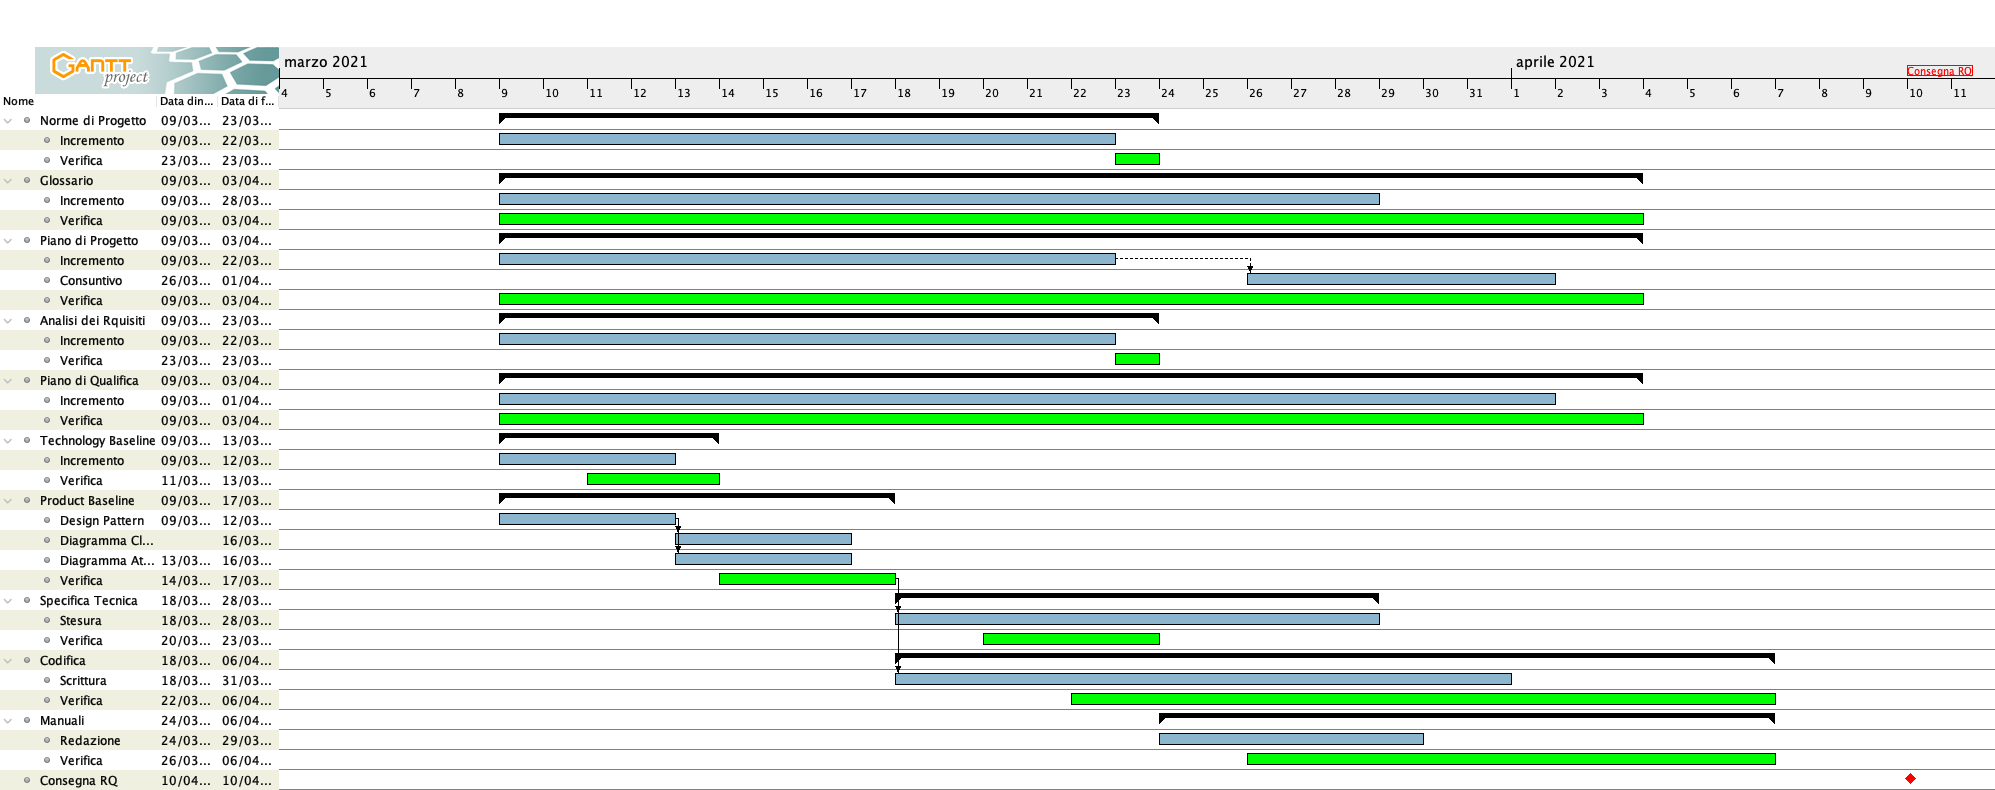
\includegraphics[width=\textwidth]{Immagini/GanttProgettazioneDiDettaglioECodifica}
    \caption{Diagramma di Gantt dell'attività di progettazione di dettaglio e codifica}
\end{figure}